\question The transition system is 

\begin{figure}[ht]
    \centering
    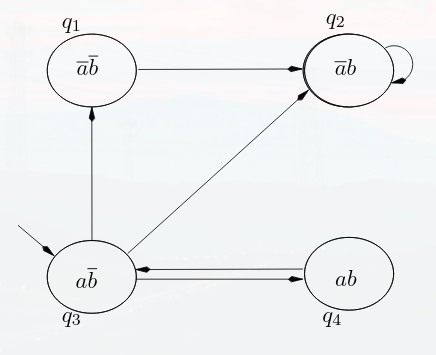
\includegraphics[width=0.35\textwidth]{fig/q2ts.png}
    \caption{The model}
    \label{fig:q2ts}
\end{figure}

\begin{alphaparts}
    \setcounter{partCounter}{2}

    \questionpart $a \until \lnext (a \land \lnot b)$ --- A path satisfying this
    is the trivial $q_3 \leftrightarrow q_4$ loop. $q_3$ satisfies $a$ and $q_4$
    satsifies $\lnext (a \land \lnot b)$ by moving to $q_3$ again. None of the
    paths with the prefixes $q_3 \rightarrow q_1$ or $q_3 \rightarrow q_2$
    satisfy $\phi$, hence, $\model, q_3 \not \models \phi$.

    \questionpart $\lnext \lnot b \land \globally (\lnot a \lor \lnot b)$ --- A
    path satisfying this is $q_3 \rightarrow q_1 \rightarrow q_2 \leftrightarrow
    q_2$. The paths with prefix $q_3 \rightarrow q_4$ do not satisfy the first
    clause, hence, $\model, q_3 \not\models \phi$.
\end{alphaparts}